
\section{绪论/Introduction}

\subsection{Chiplet基本介绍}

Chiplet(芯粒)是一种模块化的处理器设计方法,将大型、复杂的芯片分解成多个功能独立的“芯粒”,这些芯粒使用标准化的通信接口(如 PCIe、HBM 或 AIB)连接在一个封装内,从而构建出高性能的系统级芯片(SoC)。这种架构的优势在于,可以利用不同的工艺节点生产不同功能的芯粒(异构集成),提高良率、降低成本,并缩短开发周期。

\begin{figure}[htbp]
	\centering
	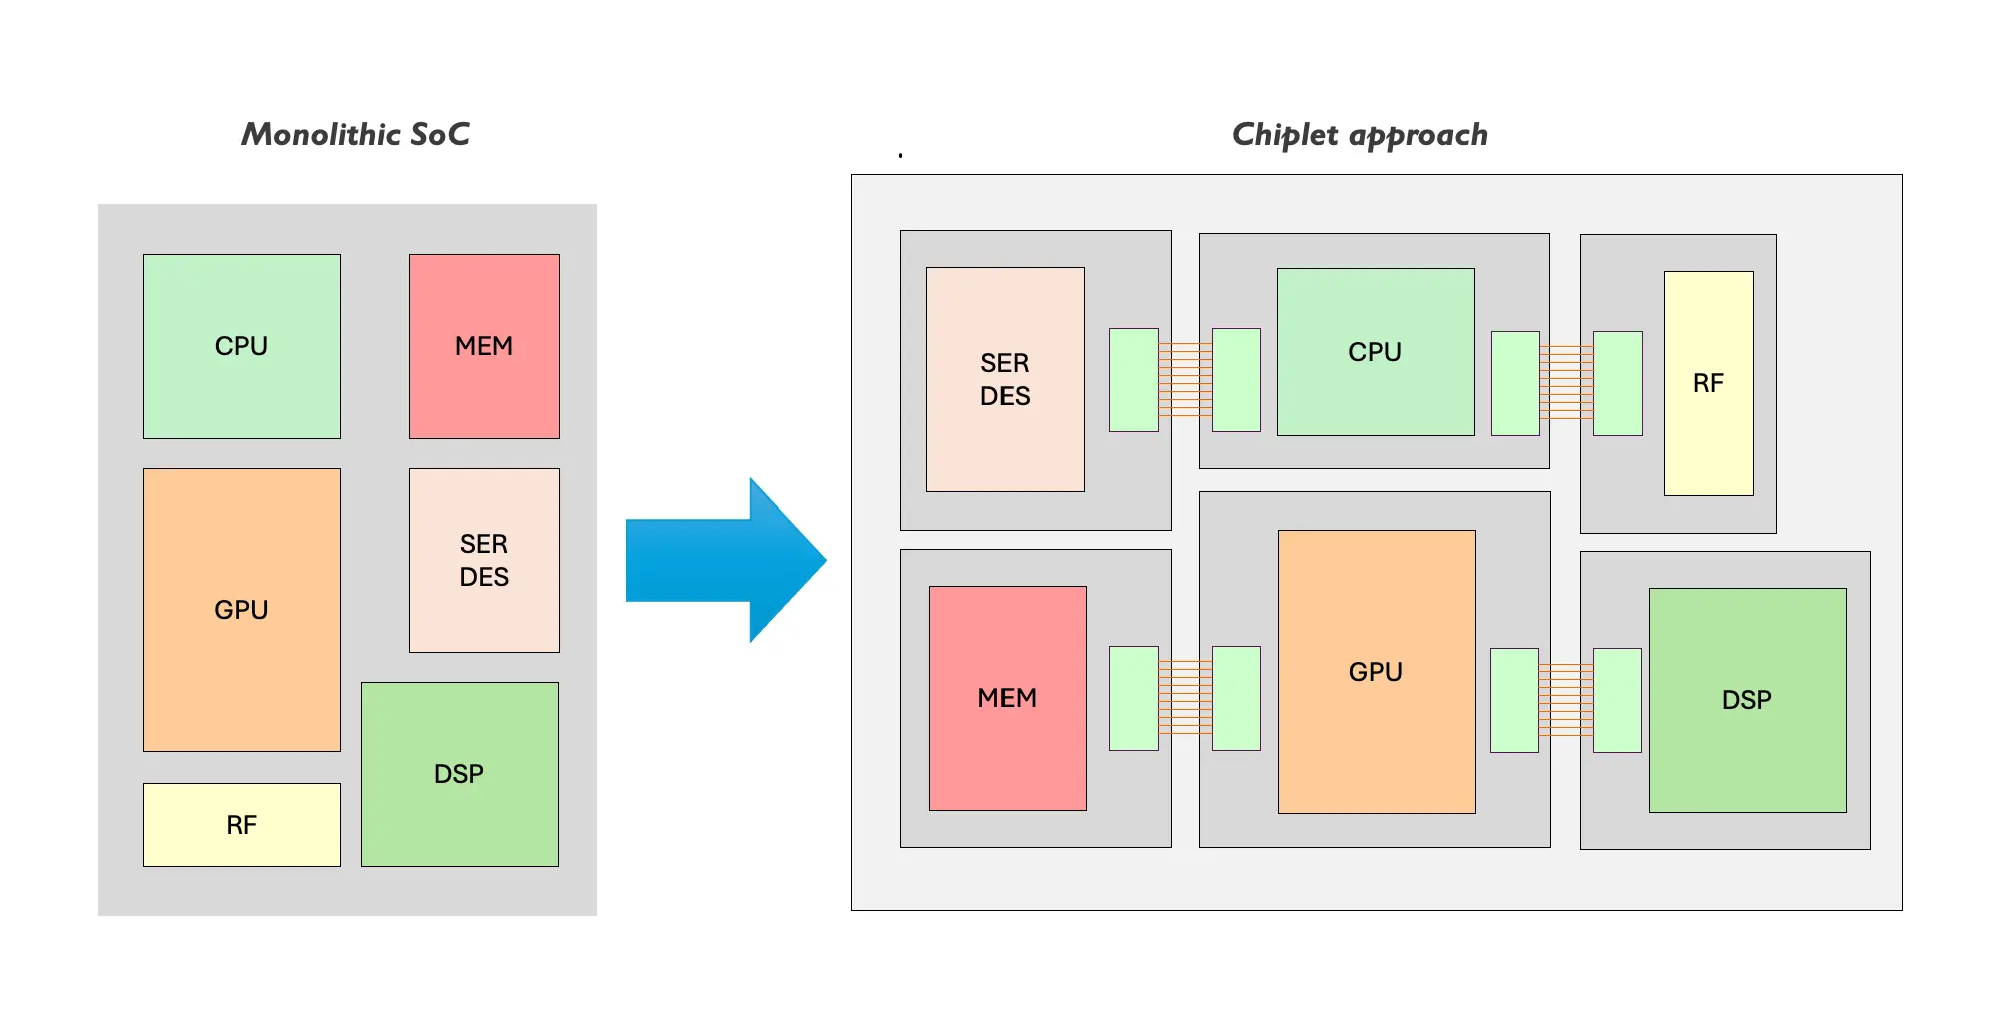
\includegraphics[width=0.8\textwidth]{img/1-1.png} % 图片文件名,不需要加扩展名
	\caption{单片集成电路片上系统与Chiplet架构系统示意图 \cite{Beyne2024Chiplet}}
	\label{fig:example}
\end{figure}

如上图所示,右侧的Chiplet架构示意图是一个微型集成电路(integrated circuit,IC),包含明确定义的功能子集。它被设计为与单个封装内插器上的其他小芯片结合在一起。一组芯粒可以在混合搭配“乐高式”堆叠组件中实现。

作为一种异构集成技术,基于芯粒的设计技术可利用先进的封装技术将不同功能的多个异构芯片集成到单个芯片中,可有效应对摩尔定律失效。随着工艺节点向前发展,成本、设计周期和复杂性急剧上升,推动业界集中芯粒领域。 芯粒可允许IC设计人员合并不同工艺节点制造的芯片,并在不同的项目中重复使用,这有助于降低设计成本,提高良率。

\subsection{采用小芯片Chiplet技术的优点}

优化性能和功耗:芯片组可以针对其特定功能和技术进行优化,从而提升系统级芯片 (SoC) 的性能和功耗。芯片组还可以更紧密地排列,从而降低互连延迟和功耗。

降低制造成本:Chiplet 可以使用不同的工艺节点和代工厂进行制造,从而降低了生产大型复杂芯片的成本和风险。Chiplet 还可以在不同的 SoC 之间重复使用,从而提高投资回报率并缩短产品上市时间。

更高的灵活性和可扩展性:芯片组可以轻松添加或移除,以调整SoC的功能和性能。芯片组的更新或替换不会影响SoC的其他部分,从而加快创新速度,并适应不断变化的市场需求。

\begin{figure}[htbp]
	\centering
	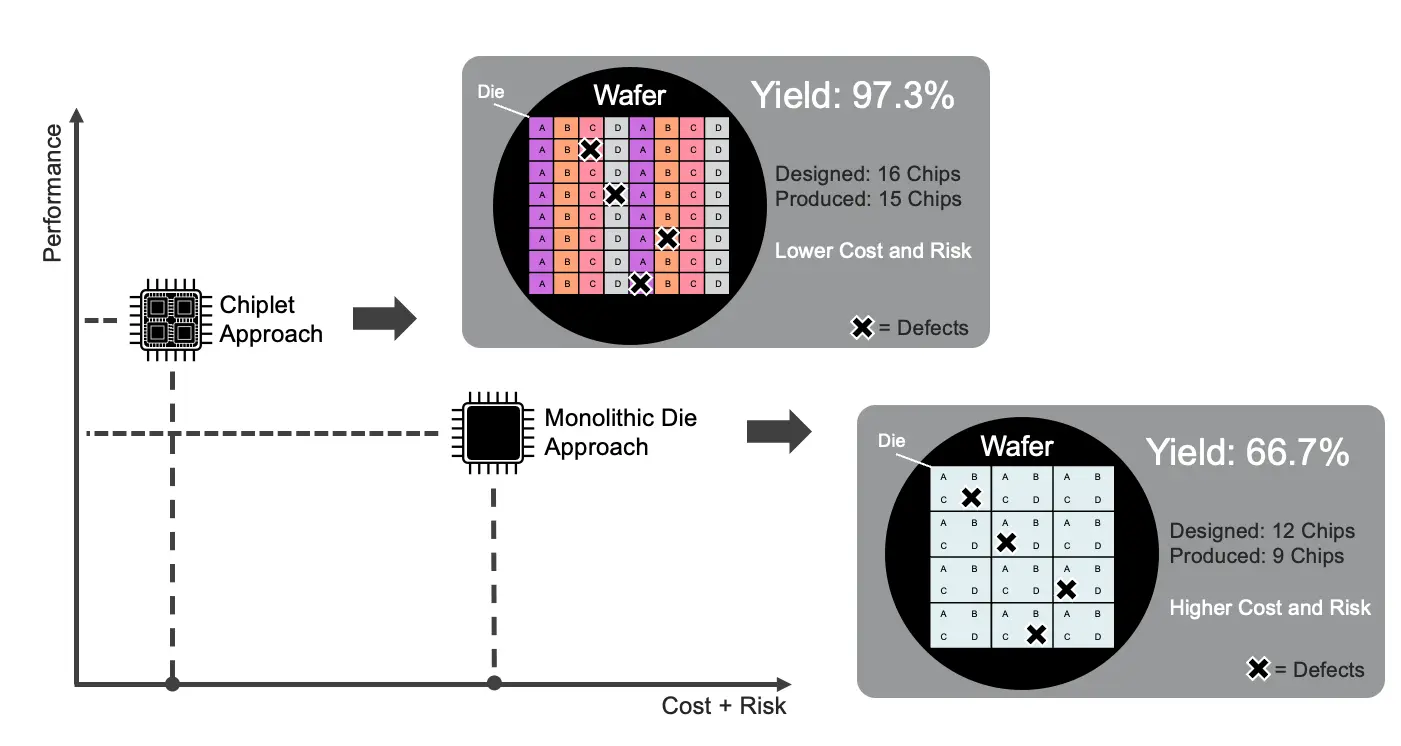
\includegraphics[width=0.8\textwidth]{img/2.png} % 图片文件名,不需要加扩展名
	\caption{小芯片与单片芯片方法的性能和成本比较 \cite{PiacentiniFilho2024Chiplet}}
	\label{fig:example}
\end{figure}

\pagebreak

\subsection{Chiplet设计的挑战}

虽然 Chiplet 的模块化方法提高了良率,但功能模块现在位于不同的芯片上,通常来自不同的供应商。设计人员无法深入探究 SoC 中每个功能 Chiplet 的内部,这增加了设计复杂性。先进的仿真和采用支持 Chiplet 工作流程的现代 EDA 解决方案成为解决这一问题的关键。

Chiplet 设计的另一个主要挑战是 Chiplet 之间的通信,即芯片间 (D2D) 通信。稳健且标准化的 D2D 通信对于确保 Chiplet 设计的可靠性和互操作性至关重要。UCIe 是一个正在兴起的开放标准,旨在标准化 D2D 通信并提高 Chiplet 设计的可靠性和互操作性。